\documentclass[a4paper, 12pt]{article}

\usepackage{babel}
\usepackage{enumitem}
\usepackage{times}
\usepackage{graphicx}
\usepackage{geometry}
	\geometry{left = 4cm, top = 4cm, right = 3cm, bottom = 3cm}
\usepackage{float}
\usepackage{setspace}
	\setstretch{1.5}
\usepackage{listings}


\begin{document}
\title{\textbf{Tugas Modul Praktikum Pemrograman II}}
\date{}

\maketitle

\begin{figure}[!ht]
\begin{center}

\includegraphics[width = 4cm, height = 3.5cm]{gambar/logo.png}
\end{center}
\end{figure}

\begin{center}
\vspace{1cm}
Disusun Oleh:\\
Faris Muhammad Ihsan\\
D4 TI 2B\\
1.18.4.099\\
\vspace{1cm}
\textbf{PROGRAM DIPLOMA IV POLITEKNIK POS INDONESIA} \linebreak
\textbf{POLITEKNIK POS INDONESIA} \linebreak
\textbf{BANDUNG}\linebreak
\textbf{2019}

\end{center}

\thispagestyle{empty}

\clearpage
\setcounter{page}{1}

\begin{center}
\title{\LARGE \bf Chapter 3}\\
\title{\LARGE \bf Pemrograman Dasar}\\
\end{center}

\appendix
\section{Teori}

\begin{enumerate}
\item Fungsi\\
Fungsi : bagian dari program yang dapat digunakan ulang untuk melakukan sebuah tindakan.fungsi dapat dipanggil pada fungsi lain, fungsi pada python yaitu def.\\
Inputan fungsi : untuk mengambil data\\
Contoh :\\
\lstinputlisting[language=Python]{src/1.py}

\item Paket\\
Paket : modul yang berisi kode-kode dan bisa di impor kedalam program\\
Cara pemanggilan paket : \\
\lstinputlisting[language=Python]{src/2.py}

\item Kelas, objek, atribut, method\\
Kelas : sebuah blueprint dari sebuah objek\\
contoh :\\
 class syabriena:\\

Objek : hasil cetak dari kelas\\
Contoh :  \\
class TI:
	dari\textunderscore kelas = "2B"
syabriena = TI()

Atribut : variabel yang dideklarasikan\\
Contoh : \\

Method : fungsi pada objek.\\
Contoh : \\

\item Cara pemanggilan library\\
Contoh :\\
\lstinputlisting[language=Python]{src/4.py}

\item Pemakaian paket dengan from kalkulator import penambahan\\
\lstinputlisting[language=Python]{src/5.py}

\item Paket fungsi apabila file library ada di dalam folder\\
\lstinputlisting[language=Python]{src/6.py}

\item  Paket kelas apabila file library ada di dalam folder\\
\lstinputlisting[language=Python]{src/7.py}

\end{enumerate}

\section{Keterampilan Pemrograman}

\begin{enumerate}
\item Soal 1
\lstinputlisting[language=Python]{src/NPM(1).py}

\item Soal 2
\lstinputlisting[language=Python]{src/NPM(2).py}

\item Soal 3
\lstinputlisting[language=Python]{src/NPM(3).py}

\item Soal 4
\lstinputlisting[language=Python]{src/NPM(4).py}

\item Soal 5
\lstinputlisting[language=Python]{src/NPM(5).py}

\item Soal 6
\lstinputlisting[language=Python]{src/NPM(6).py}

\item Soal 7
\lstinputlisting[language=Python]{src/NPM(7).py}

\item Soal 8
\lstinputlisting[language=Python]{src/NPM(8).py}

\item Soal 9
\lstinputlisting[language=Python]{src/NPM(9).py}

\item Soal 10
\lstinputlisting[language=Python]{src/NPM(10).py}

\item Soal 11
\lstinputlisting[language=Python]{src/lib3.py}

\item Soal 12
\lstinputlisting[language=Python]{src/kelas3lib.py}

\section{Keterampilan Penanganan Error}
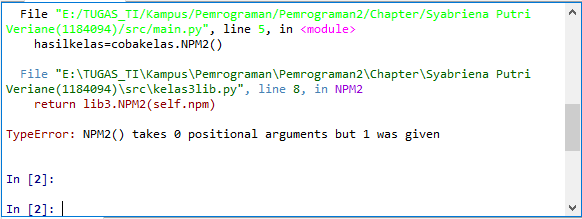
\includegraphics{gambar/error3.png}
Solusi : tambahkan parameter pada fungsi NPM2().\\

Try Except:
\lstinputlisting[language=Python]{src/tryexcept.py}

\end{enumerate}











\end{document}

